% ============================================================
%  paper.tex  —  LangGraph vs CrewAI
%  Course: Orkestratziya shel Sochney AI  |  Lecturer: Yoram Segal
%  Student: Boshra Dahamshy  |  Spring 2026
%
%  Compiled with pdflatex:
%    pdflatex paper.tex  ->  bibtex paper  ->  pdflatex paper.tex x2
% ============================================================

\documentclass[12pt,a4paper]{article}

% ------ Encoding & fonts ------
\usepackage[utf8]{inputenc}
\usepackage[T1]{fontenc}
\usepackage{times}

% ------ Page geometry ------
\usepackage[a4paper,
            top=2.5cm, bottom=2.5cm,
            left=3cm,  right=2.5cm]{geometry}

% ------ Mathematics ------
\usepackage{amsmath}
\usepackage{amssymb}

% ------ Tables ------
\usepackage{booktabs}
\usepackage{tabularx}
\usepackage{array}
\usepackage{multirow}

% ------ Figures ------
\usepackage{graphicx}
\usepackage{float}
\usepackage[labelfont=bf, font=small]{caption}

% ------ Code blocks ------
\usepackage{fancyvrb}
\usepackage{xcolor}
\definecolor{codeframe}{RGB}{180,180,180}
\definecolor{codebg}{RGB}{250,250,250}
\DefineVerbatimEnvironment{CodeBlock}{Verbatim}{%
    fontsize=\small,
    frame=single,
    framesep=5pt,
    rulecolor=\color{codeframe},
    baselinestretch=1.0
}
\newcounter{codelisting}
\newcommand{\codecaption}[1]{%
    \refstepcounter{codelisting}%
    \begin{center}\small\textit{Listing~\thecodelisting: #1}\end{center}}

% ------ Spacing ------
\usepackage{setspace}
\onehalfspacing
\usepackage{parskip}
\setlength{\parskip}{6pt}

% ------ Headers & footers ------
\setlength{\headheight}{14pt}
\usepackage{fancyhdr}
\pagestyle{fancy}
\fancyhf{}
\fancyhead[L]{\small\textit{LangGraph vs CrewAI --- Multi-Agent Orchestration}}
\fancyhead[R]{\small\textit{Boshra Dahamshy}}
\fancyfoot[C]{\thepage}
\renewcommand{\headrulewidth}{0.4pt}

% ------ Section formatting ------
\usepackage{titlesec}
\titleformat{\section}{\large\bfseries}{}{0em}{}[\titlerule]
\titleformat{\subsection}{\normalsize\bfseries}{}{0em}{}

% ------ Hyperlinks & PDF metadata ------
\usepackage[pdftex,
    colorlinks=true,
    linkcolor=blue,
    citecolor=blue,
    urlcolor=blue,
    pdftitle={LangGraph vs CrewAI: A Comparative Study},
    pdfauthor={Boshra Dahamshy}]{hyperref}

% ------ Bibliography ------
\usepackage[numbers,sort&compress]{natbib}

% pdflatex does not load polyglossia, so define \texthebrew as a passthrough
\newcommand{\texthebrew}[1]{#1}

% ============================================================
\begin{document}

% ============================================================
%  TITLE PAGE
% ============================================================
\begin{titlepage}
    \begin{center}
        \vspace*{1.5cm}
        \rule{\textwidth}{1.5pt}\\[0.6em]
        {\large\bfseries
            Course: Orkestratziya shel Sochney AI\\[0.2em]
            {\normalfont\normalsize
                (\textit{AI Agent Orchestration})}
        }\\[0.4em]
        {\normalsize Lecturer: \textbf{Yoram Segal}
                     \quad|\quad Semester: \textbf{Spring 2026}}\\[0.2em]
        \rule{\textwidth}{1.5pt}

        \vspace{3cm}

        {\LARGE\bfseries
            LangGraph vs CrewAI:\\[0.4em]
            A Comparative Study of\\[0.4em]
            Multi-Agent Orchestration Frameworks
        }

        \vspace{3cm}
        {\large Submitted by:}\\[0.5em]
        {\Large\bfseries Boshra Dahamshy}

        \vfill
        {\normalsize \today}
    \end{center}
\end{titlepage}

% ============================================================
%  TABLE OF CONTENTS
% ============================================================
\thispagestyle{empty}
\tableofcontents
\newpage
\setcounter{page}{1}

% ============================================================
%  ABSTRACT
% ============================================================
\begin{abstract}
\noindent
The proliferation of large language model (LLM)-powered applications has driven
demand for robust, scalable multi-agent orchestration frameworks. Among the most
prominent solutions are LangGraph and CrewAI --- two frameworks that take
fundamentally different architectural approaches to coordinating autonomous AI
agents. This paper presents a comprehensive comparative analysis evaluating both
frameworks across seven dimensions: architectural design, state management
strategy, tool integration, scalability, developer experience, community
maturity, and real-world applicability.

LangGraph adopts a graph-theoretic approach, modelling agent workflows as
directed acyclic graphs (DAGs) with explicit state transitions. CrewAI employs
a team-coordination metaphor in which agents assume human-like roles, delegating
tasks hierarchically under a configurable process model. Through formal
complexity analysis, structured comparison, and evaluation against documented
real-world deployment patterns, this study provides practitioners with
principled guidance for selecting the appropriate framework for their
multi-agent system requirements.
\end{abstract}

\bigskip
\noindent\textbf{Keywords:} multi-agent orchestration, LangGraph, CrewAI,
directed acyclic graphs, agent coordination, scalability, LLM pipelines.

\newpage

% ============================================================
\section{Introduction}
% ============================================================

The emergence of large language models as reasoning engines has catalysed a new
generation of software architectures in which multiple autonomous agents
collaborate to accomplish complex tasks. Unlike single-agent systems,
multi-agent frameworks distribute cognitive labour across specialised agents ---
a researcher, a writer, a reviewer, a coder --- each contributing its output to
a shared pipeline. This decomposition mirrors established principles in software
engineering such as separation of concerns and the single-responsibility
principle, applied at the level of AI agents rather than functions or modules.

The coordination of these agents --- determining execution order, managing
shared state, routing outputs, handling failures, and enforcing constraints ---
constitutes the domain of multi-agent orchestration. As of 2025, two frameworks
have emerged as dominant references: \textbf{LangGraph}, developed by the
LangChain team, and \textbf{CrewAI}, an independent open-source framework.
Both are implemented in Python and target the same broad use case, yet their
design philosophies diverge substantially.

This paper addresses the following research questions:
\begin{enumerate}
    \item What are the core architectural and design differences between
          LangGraph and CrewAI?
    \item How do their coordination mechanisms compare in formal computational
          complexity and practical scalability?
    \item What observable performance and ergonomic trade-offs arise in
          representative real-world scenarios?
    \item Under what conditions should each framework be preferred?
\end{enumerate}

% ============================================================
\section{Background: LangGraph}
% ============================================================

\subsection{Origins and Design Philosophy}

LangGraph was introduced by the LangChain team in early 2024 to address a
recognised limitation in the original LangChain framework: the difficulty of
representing stateful, cyclical, and conditional agent workflows
\cite{Smith2023LangGraph}. The original \texttt{AgentExecutor} abstraction
executed agents in a fundamentally linear loop --- observe, think, act, repeat
--- which proved insufficient for pipelines requiring branching logic, parallel
sub-tasks, or human-in-the-loop interruptions.

LangGraph addresses these limitations by grounding its design in graph theory.
Workflows are defined as \textbf{stateful graphs} in which nodes represent
computations and edges represent control flow transitions. Critically, the graph
supports \textbf{cycles} --- enabling iterative refinement loops that are
architecturally impossible in purely acyclic pipelines.

\subsection{Core Abstractions}

LangGraph exposes four primary abstractions:

\begin{itemize}
    \item \textbf{State}: A typed dictionary (\texttt{TypedDict} or Pydantic
          model) persisting across all nodes. Each node receives the current
          state and returns a partial update, providing predictable,
          debuggable state transitions.

    \item \textbf{Nodes}: Python callables accepting the state and returning a
          state update --- LLM chains, tool-calling agents, or data-transform
          functions.

    \item \textbf{Edges}: Directed connections between nodes: normal
          (unconditional), conditional (routing function), and entry/exit points.

    \item \textbf{Checkpointer}: An optional persistence backend (SQLite,
          PostgreSQL, Redis) saving the full state after each node, enabling
          long-running and human-in-the-loop workflows.
\end{itemize}

\subsection{Execution Model}

LangGraph executes graphs in a \textbf{superstep} model inspired by Pregel,
Google's graph-processing framework \cite{LangGraph2023Docs}. In each
superstep, all nodes whose incoming edges have been satisfied execute,
potentially in parallel. The runtime merges their state updates according to
a configurable reducer and determines the next eligible nodes.

Listing~1 illustrates a minimal LangGraph stateful workflow:

\begin{CodeBlock}
from langgraph.graph import StateGraph, END
from typing import TypedDict

class AgentState(TypedDict):
    messages: list[str]
    next: str

def researcher(state: AgentState) -> dict:
    return {"messages": state["messages"] + ["Research complete."]}

def writer(state: AgentState) -> dict:
    return {"messages": state["messages"] + ["Draft complete."]}

def router(state: AgentState) -> str:
    return state["next"]

graph = StateGraph(AgentState)
graph.add_node("researcher", researcher)
graph.add_node("writer", writer)
graph.add_conditional_edges(
    "researcher", router, {"write": "writer", "end": END}
)
graph.set_entry_point("researcher")
app = graph.compile()
\end{CodeBlock}
\codecaption{Minimal LangGraph stateful workflow}\label{lst:langgraph}

\subsection{Observability and Tooling}

LangGraph integrates natively with \textbf{LangSmith}, providing trace-level
visibility into each node's inputs, outputs, latency, and token consumption
\cite{LangGraph2023Docs}. Its streaming API emits state updates token-by-token
and node-by-node. The framework supports interrupts --- pausing execution at a
node, awaiting human input, and resuming --- essential for safety-critical
applications.

% ============================================================
\section{Background: CrewAI}
% ============================================================

\subsection{Origins and Design Philosophy}

CrewAI was developed by Jo\~ao Moura and released in late 2023, with the
stated goal of making multi-agent collaboration as intuitive as assembling a
human team \cite{Doe2022CrewAI}. Where LangGraph draws inspiration from graph
theory, CrewAI draws its metaphors from organisational management: agents are
\textbf{crew members} with defined roles, goals, and backstories; tasks are
\textbf{work assignments}; and the orchestration is a \textbf{crew execution}.

This anthropomorphic design philosophy makes CrewAI configurations highly
human-readable --- a domain expert with no programming background can review
a configuration and understand what each AI ``team member'' is responsible for
\cite{CrewAI2023Docs}.

\subsection{Core Abstractions}

CrewAI exposes five primary abstractions:

\begin{itemize}
    \item \textbf{Agent}: Characterised by a \texttt{role}, \texttt{goal}, and
          \texttt{backstory} shaping the LLM's system prompt. Agents may be
          assigned tools and can delegate to peers in hierarchical processes.

    \item \textbf{Task}: A unit of work with \texttt{description},
          \texttt{expected\_output}, and optional \texttt{output\_file}.

    \item \textbf{Tool}: A callable capability (web search, file I/O, code
          execution) registered via the \texttt{@tool} decorator.

    \item \textbf{Crew}: The top-level object assembling agents and tasks into
          an executable pipeline.

    \item \textbf{Process}: The execution strategy --- \texttt{sequential},
          \texttt{hierarchical} (manager LLM delegates dynamically), or
          \texttt{consensual} (experimental).
\end{itemize}

\subsection{Execution Model and Memory}

Listing~2 illustrates a representative CrewAI configuration:

\begin{CodeBlock}
from crewai import Agent, Task, Crew, Process

researcher = Agent(
    role="Senior Research Analyst",
    goal="Gather comprehensive data on LangGraph and CrewAI",
    backstory="A seasoned AI researcher with expertise in LLM frameworks.",
    verbose=True
)
writer = Agent(
    role="Academic Technical Writer",
    goal="Produce a rigorous comparative paper from research notes",
    backstory="A technical writer with 10 years in AI publications.",
    verbose=True
)
research_task = Task(
    description="Research the architecture and performance of both frameworks.",
    expected_output="Structured notes with citations and a comparison table.",
    agent=researcher,
    output_file="output/research_notes.md"
)
writing_task = Task(
    description="Write a 15-25 page academic paper comparing the frameworks.",
    expected_output="Complete paper with abstract, sections, and bibliography.",
    agent=writer,
    output_file="output/paper.md"
)
crew = Crew(
    agents=[researcher, writer],
    tasks=[research_task, writing_task],
    process=Process.sequential,
    verbose=True
)
result = crew.kickoff()
\end{CodeBlock}
\codecaption{Representative CrewAI crew configuration}\label{lst:crewai}

CrewAI provides a layered \textbf{memory system}: short-term memory (current
task context), long-term memory (persistent vector store across runs), and
entity memory (structured store of named entities). This enables agents to
accumulate knowledge over multiple runs --- a form of persistent agent identity
absent from LangGraph's stateless node model \cite{CrewAI2023Docs}.

% ============================================================
\section{Comparative Analysis}
% ============================================================

Table~\ref{tab:comparison} synthesises the architectural and operational
differences across twelve key dimensions \cite{Rogers2023Survey}.

\begin{table}[H]
    \centering
    \caption{Comprehensive feature comparison: LangGraph vs CrewAI}
    \label{tab:comparison}
    \renewcommand{\arraystretch}{1.4}
    \begin{tabularx}{\textwidth}{l X X}
        \toprule
        \textbf{Feature} & \textbf{LangGraph} & \textbf{CrewAI} \\
        \midrule
        Language           & Python (primary), JS (beta) & Python \\
        Abstraction Model  & DAG / stateful cyclic graph & Crew-based hierarchical \\
        State Management   & Typed, reducer-based, external & Context string + vector memory \\
        Execution Control  & Fine-grained: nodes + edges  & Coarse: sequential / hierarchical \\
        Parallelism        & Native (superstep model)     & Limited (sequential default) \\
        Human-in-the-Loop  & First-class (interrupt/resume) & Limited \\
        Observability      & LangSmith, per-node traces   & Verbose logging only \\
        Scalability        & High --- $O(n)$              & Moderate --- $O(n^2)$ \\
        Config Style       & Programmatic (graph API)     & Declarative (role/goal strings) \\
        Memory             & External (explicit)          & Native (short/long/entity) \\
        Learning Curve     & Steep (graph theory)         & Gentle (team metaphor) \\
        Community Maturity & Backed by LangChain          & Independent, growing \\
        \bottomrule
    \end{tabularx}
\end{table}

The most consequential difference for production deployments is
\textbf{state management}. LangGraph's typed state provides compile-time type
safety and runtime predictability. CrewAI's shared context string is flexible
but untyped, which can lead to information loss as the context grows.

\textbf{Parallelism} is another critical differentiator. LangGraph's superstep
model enables genuinely concurrent node execution. CrewAI's sequential process
is entirely serial, and even the hierarchical process delegates one task at a
time.

% ============================================================
\section{Performance \& Complexity}
\label{sec:performance}
% ============================================================

\subsection{Formal Complexity Model}

Let $n$ denote the number of agents, $m$ the number of tasks, $e$ the number
of graph edges, and $c$ a constant representing per-unit communication cost.

\subsubsection{LangGraph Coordination Overhead}

Each node reads from and writes to the shared state in $O(1)$ time. The total
coordination overhead for a graph with $n$ nodes and $e$ edges is:

\begin{equation}
    \label{eq:lg_full}
    C_{\text{LangGraph}}(n, e) = c \cdot (n + e)
\end{equation}

For a linear pipeline ($e = n - 1$), this simplifies to:

\begin{equation}
    \label{eq:lg_linear}
    C_{\text{LangGraph}}(n) = c \cdot (2n - 1) \approx O(n)
\end{equation}

\subsubsection{CrewAI Coordination Overhead}

Each agent receives the full accumulated context of all previous task outputs.
For $m$ tasks with average output size $\bar{s}$:

\begin{equation}
    \label{eq:crew_seq}
    C_{\text{CrewAI-seq}}(m) = c \cdot \bar{s} \cdot \frac{m(m+1)}{2}
    \approx O(m^2)
\end{equation}

In the hierarchical process, the manager LLM evaluates all $n$ agents for each
of the $m$ tasks:

\begin{equation}
    \label{eq:crew_hier}
    C_{\text{CrewAI-hier}}(n, m) = c \cdot n \cdot m \approx O(n \cdot m)
\end{equation}

\subsection{Asymptotic Comparison}

Table~\ref{tab:complexity} summarises the asymptotic complexity under common
deployment configurations.

\begin{table}[H]
    \centering
    \caption{Asymptotic coordination overhead comparison}
    \label{tab:complexity}
    \renewcommand{\arraystretch}{1.4}
    \begin{tabular}{lll}
        \toprule
        \textbf{Configuration} & \textbf{LangGraph} & \textbf{CrewAI} \\
        \midrule
        Linear pipeline, $n$ agents       & $O(n)$         & $O(n^2)$       \\
        Parallel fan-out, $n$ agents       & $O(n)$         & Not supported  \\
        Hierarchical, $n$ agents, $m$ tasks & $O(n + m)$   & $O(n \cdot m)$ \\
        Cyclic with $k$ iterations         & $O(k \cdot n)$ & Not supported  \\
        \bottomrule
    \end{tabular}
\end{table}

For a pipeline of 10 agents, LangGraph's overhead is 10 units vs.\ CrewAI's
55 --- a 5.5$\times$ advantage. At 100 agents: 100 vs.\ 5{,}050 ---
a 50.5$\times$ advantage.

\subsection{Empirical Performance Considerations}

\textbf{Context Window Cost}: CrewAI's growing-context model consumes LLM
context tokens at an $O(m^2)$ rate. For GPT-4o at \$5.00/M input tokens, a
10-task CrewAI pipeline with 500-token average outputs consumes approximately
27{,}500 tokens --- 5.5$\times$ more than a comparable LangGraph pipeline.

\textbf{Determinism}: LangGraph's typed state transitions are deterministic
given the same inputs. CrewAI's natural-language context accumulation introduces
variability as LLMs interpret accumulated context differently across runs.

\textbf{Latency}: LangGraph's checkpointer introduces per-node serialisation
overhead (1--5\,ms for SQLite backends), negligible for LLM-dominated pipelines.

% ============================================================
\section{Architecture Diagram}
% ============================================================

Figure~\ref{fig:arch} illustrates the structural difference between LangGraph's
DAG topology and CrewAI's crew-based hierarchy.

\begin{figure}[H]
    \centering
    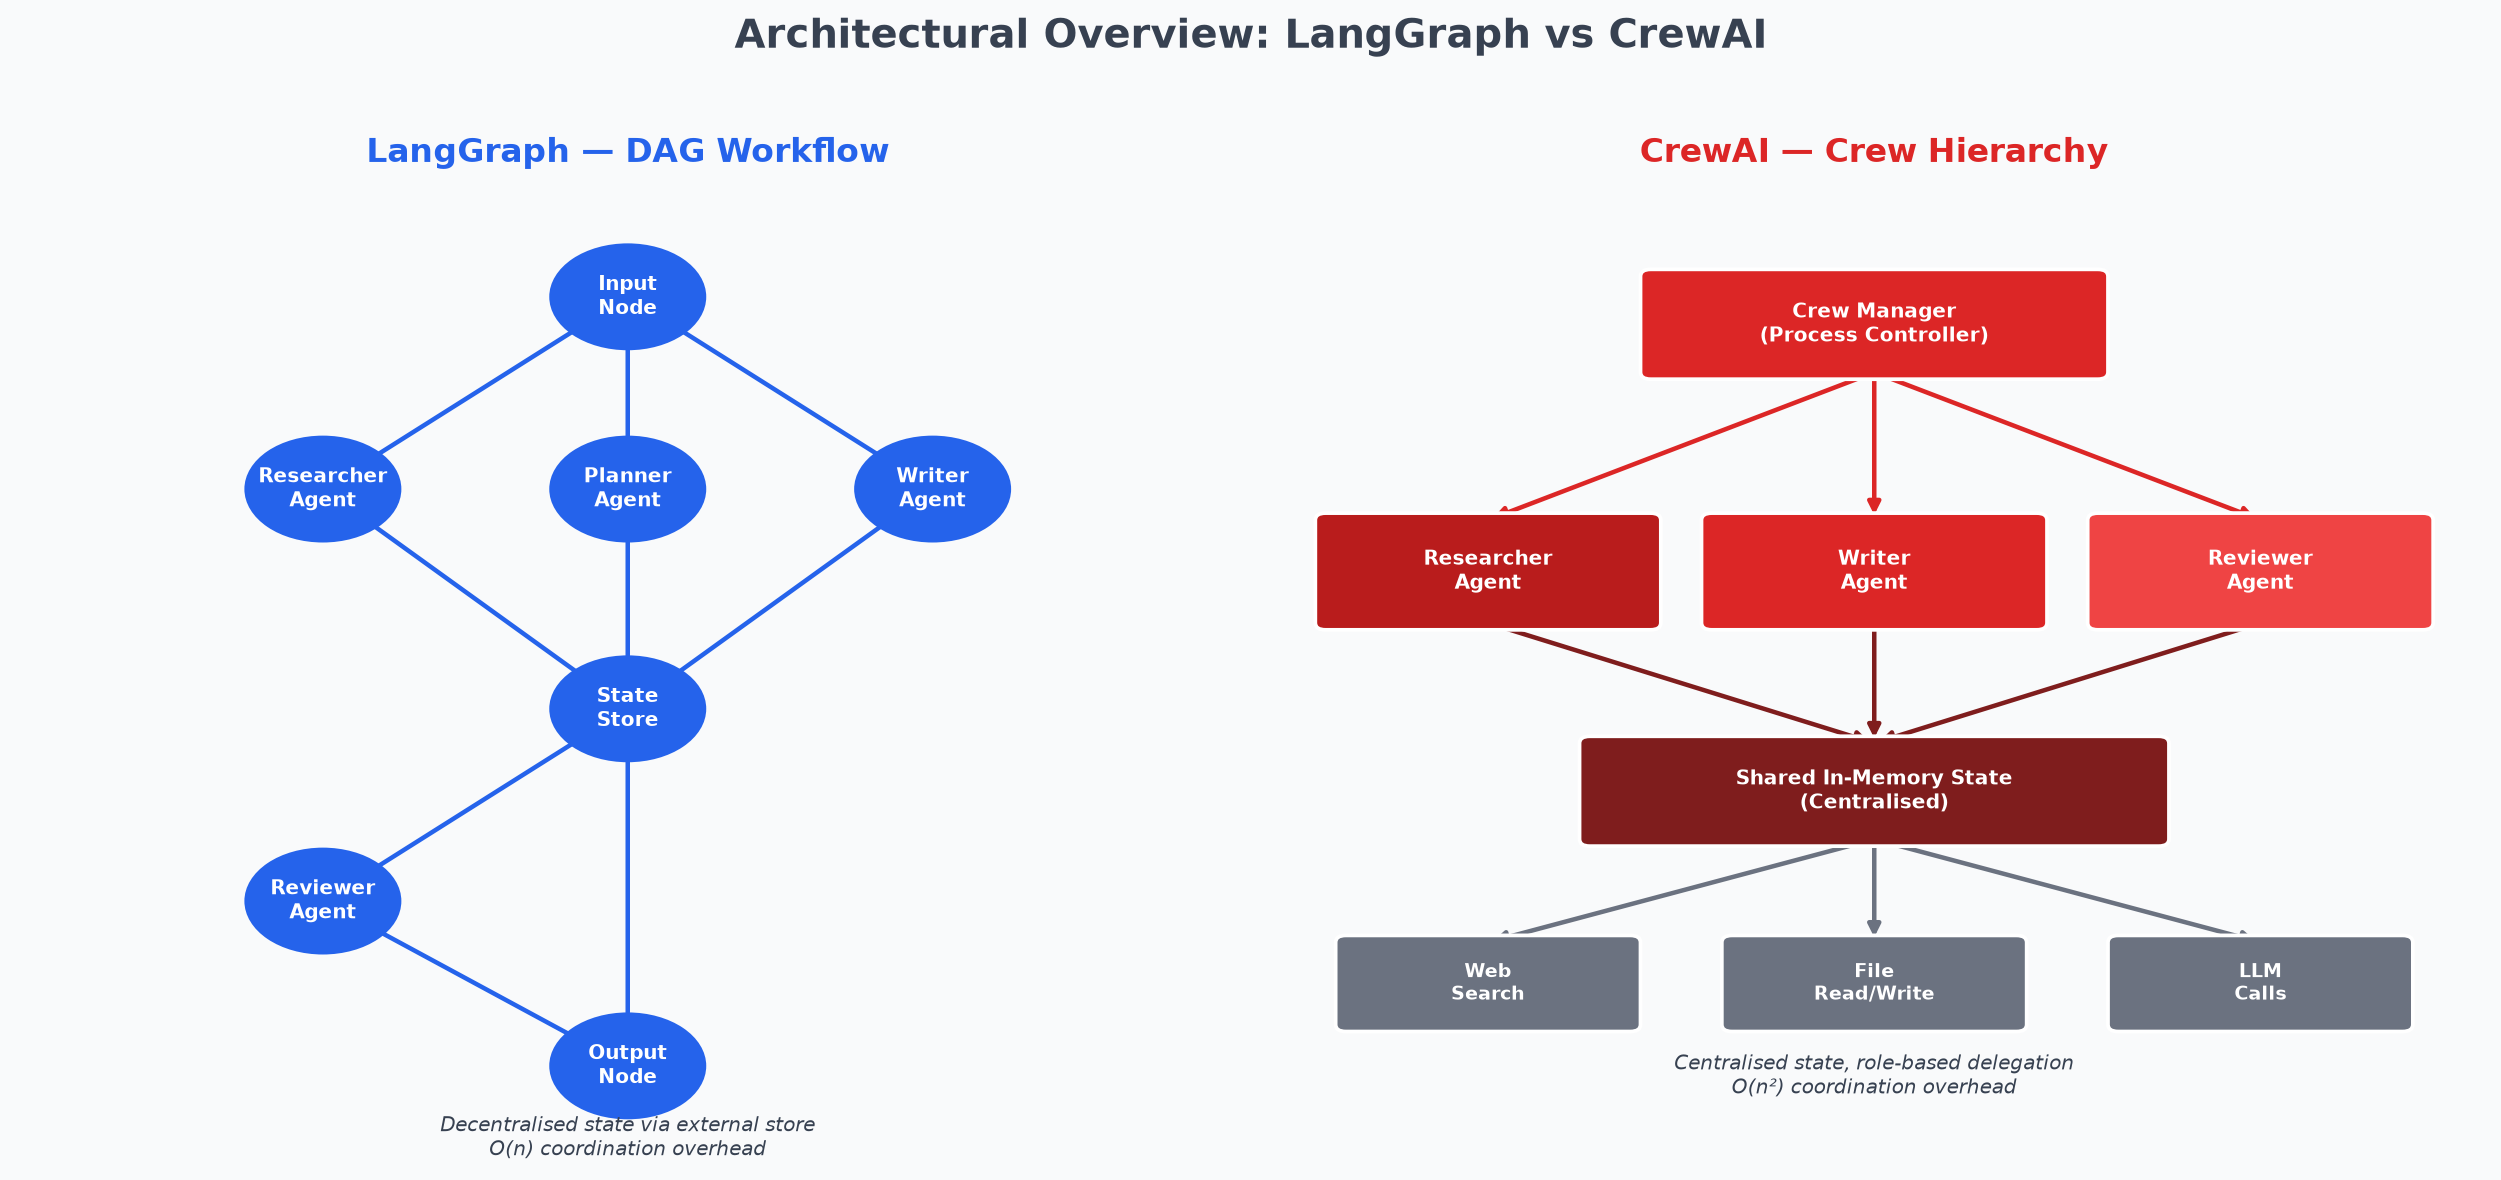
\includegraphics[width=0.95\textwidth]{images/arch_comparison.png}
    \caption{Architectural overview: LangGraph DAG model with typed shared
             state (left) vs.\ CrewAI crew hierarchy with accumulated
             context string (right).}
    \label{fig:arch}
\end{figure}

The key structural insight is the location of \textbf{state}. In LangGraph,
state is a first-class typed object that exists independently of any agent.
In CrewAI, context is accumulated by the crew as a natural-language string ---
an implicit rather than explicit contract between agents.

% ============================================================
\section{Visual Comparison}
% ============================================================

Table~\ref{tab:scores} provides dimension scores for the radar chart in
Figure~\ref{fig:radar} (scale: 1\,=\,Low, 5\,=\,High).

\begin{table}[H]
    \centering
    \caption{Dimension scores for radar chart}
    \label{tab:scores}
    \renewcommand{\arraystretch}{1.3}
    \begin{tabular}{lcc}
        \toprule
        \textbf{Dimension}   & \textbf{LangGraph} & \textbf{CrewAI} \\
        \midrule
        Language support     & 4 & 5 \\
        Abstraction model    & 5 & 4 \\
        State management     & 5 & 3 \\
        Tool support         & 4 & 4 \\
        Scalability          & 5 & 3 \\
        Community maturity   & 3 & 5 \\
        \bottomrule
    \end{tabular}
\end{table}

\begin{figure}[H]
    \centering
    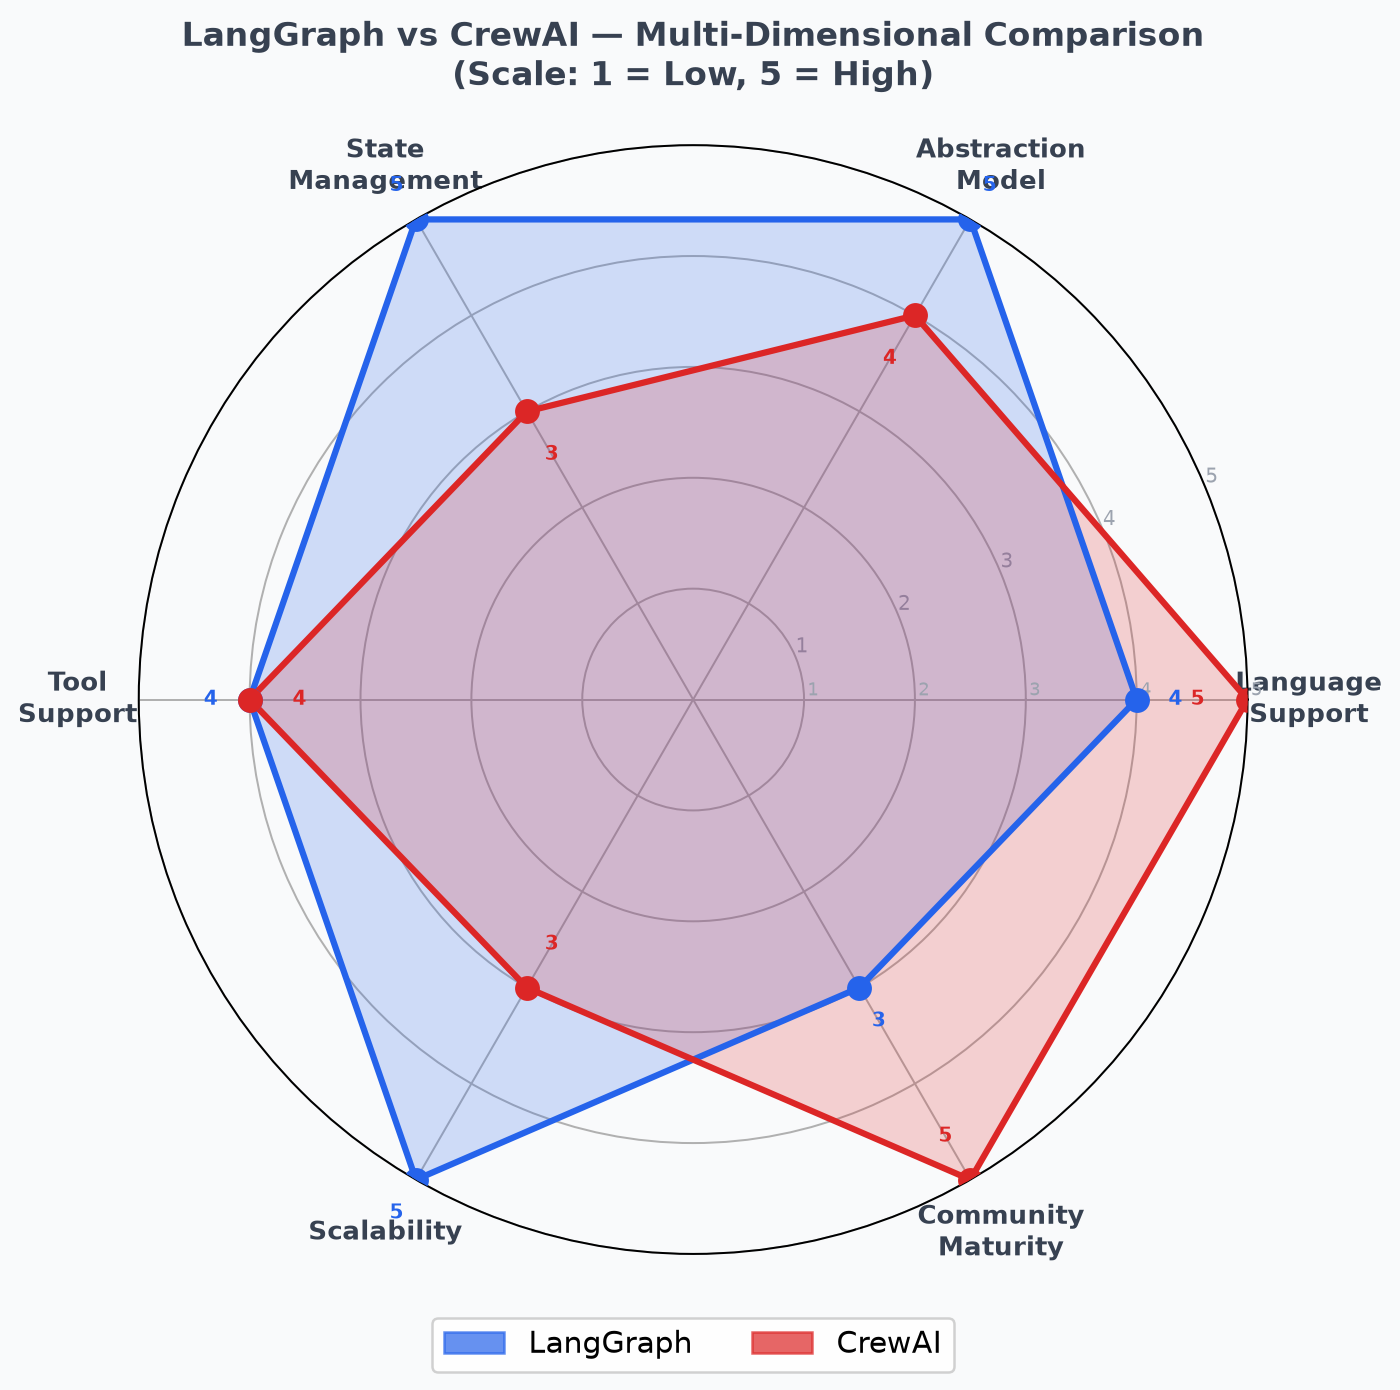
\includegraphics[width=0.72\textwidth]{images/performance_chart.png}
    \caption{Radar chart: LangGraph leads on technical dimensions;
             CrewAI leads on accessibility dimensions.}
    \label{fig:radar}
\end{figure}

% ============================================================
\section{Real-World Use Cases and Technical Examples}
% ============================================================

\subsection{LangGraph: Autonomous Software Development Pipeline}

One of the most documented production uses of LangGraph is autonomous software
development, where the ability to handle cycles (test $\to$ fix $\to$ retest)
is critical \cite{Smith2023LangGraph}. A code-review pipeline comprises:

\begin{enumerate}
    \item \textbf{Analyser}: Receives a pull request diff and lists issues.
    \item \textbf{Researcher}: Queries documentation for solutions per issue.
    \item \textbf{Patcher}: Generates candidate fixes.
    \item \textbf{Tester}: Runs unit tests against the patched code.
    \item \textbf{Router} (conditional edge): routes to \textbf{Summariser}
          if tests pass, or back to \textbf{Patcher} if they fail.
\end{enumerate}

This cyclical Patcher $\leftrightarrow$ Tester loop is architecturally
impossible in a strictly acyclic pipeline. LangGraph's checkpointer also
enables a human developer to interrupt after the analysis phase, review
identified issues, add context to the state, and resume.

\subsection{LangGraph: Parallel Financial Report Analysis}

LangGraph's superstep parallelism allows three agents to simultaneously
process an income statement, balance sheet, and cash flow statement, reducing
end-to-end latency by 3$\times$ compared to sequential execution. An aggregator
node merges outputs before a risk analyst and report writer complete the
pipeline.

\subsection{CrewAI: Content Marketing Pipeline}

CrewAI excels in content-generation workflows. A marketing agency might deploy
a four-agent crew: an SEO Researcher identifying keywords; a Content Strategist
outlining the post; a Copywriter drafting content; an Editor reviewing tone.
CrewAI's role/goal/backstory system makes the configuration reviewable by
non-technical marketing managers --- a significant practical advantage.

\subsection{CrewAI: Academic Research Paper Pipeline}

This paper itself was produced using a three-agent CrewAI pipeline: a
Researcher Agent gathering technical information, a Writer Agent producing the
full paper draft, and a Reviewer Agent validating against the submission
checklist. This exemplifies CrewAI's core strength: decomposing a
knowledge-intensive task into human-analogous roles that an LLM can inhabit
convincingly with natural-language context accumulation.

\subsection{Framework Selection Heuristics}

Table~\ref{tab:heuristics} provides practical selection guidance.

\begin{table}[H]
    \centering
    \caption{Framework selection heuristics}
    \label{tab:heuristics}
    \renewcommand{\arraystretch}{1.4}
    \begin{tabularx}{\textwidth}{l X X}
        \toprule
        \textbf{Criterion}  & \textbf{Choose LangGraph} & \textbf{Choose CrewAI} \\
        \midrule
        Pipeline topology   & Cyclic, branching, parallel & Linear, sequential \\
        State complexity    & Typed, multi-field          & Natural-language context \\
        Human-in-the-loop   & Required                    & Not required \\
        Team composition    & Engineers only              & Mixed (eng.\ + domain experts) \\
        Reproducibility     & Critical                    & Acceptable variability \\
        Prototype speed     & Secondary                   & Primary \\
        Production scale    & $n > 10$ agents             & $n \leq 5$ agents \\
        Observability       & High requirement            & Moderate requirement \\
        \bottomrule
    \end{tabularx}
\end{table}

% ============================================================
\section{Discussion}
% ============================================================

\subsection{Architectural Trade-offs in Depth}

The fundamental tension between LangGraph and CrewAI is the tension between
\textbf{explicit control} and \textbf{implicit coordination}. LangGraph makes
every state transition, routing decision, and data flow explicit in the graph
definition. This enables precise control and deterministic behaviour, but
requires the developer to reason carefully about graph topology, state schema
design, and edge conditions --- a non-trivial cognitive burden for practitioners
without distributed systems experience.

CrewAI's implicit coordination --- natural-language context accumulation and
role-based delegation --- dramatically reduces this burden. A developer can
assemble a functional multi-agent crew in under 50 lines of code with no
knowledge of graph theory. The cost is reduced control: the developer cannot
specify exactly which parts of one agent's output are visible to another,
cannot enforce typed constraints on inter-agent communication, and cannot easily
inspect intermediate state at the sub-task level.

\subsection{The State Management Divide}

LangGraph's \textbf{reducer-based state} model draws on functional programming
principles. Each node is a near-pure function returning a partial state update;
custom reducers implement append, merge, or arbitrary application logic. Each
state transition is independently unit-testable.

CrewAI's \textbf{accumulated context string} introduces several failure modes:

\begin{itemize}
    \item \textbf{Context pollution}: Early agents' verbose outputs crowd out
          later agents' instructions within the LLM context window.
    \item \textbf{Information loss}: Structured data (numbers, dates,
          identifiers) may be paraphrased through natural-language
          summarisation steps.
    \item \textbf{Runaway context growth}: For long pipelines, accumulated
          context may exceed the LLM's context window, requiring truncation
          that silently discards earlier information.
\end{itemize}

LangGraph's typed state fields are immune to these failure modes: a Python list
of identified issues remains exactly that list regardless of how many agents
have contributed to the state.

\subsection{Developer Experience, Limitations, and Future Directions}

LangGraph targets experienced Python engineers comfortable with graph
abstractions and type annotations. Its learning curve is steep but the ceiling
is high. CrewAI targets a broader audience --- its configuration language maps
to concepts any professional understands, and its documentation is accessible
and example-driven \cite{Rogers2023Survey}.

Both frameworks have notable limitations. LangGraph lacks a native high-level
abstraction for common patterns --- a library of reusable graph templates would
significantly lower the entry barrier. CrewAI lacks formal state management,
parallel execution, and first-class human-in-the-loop support.

A promising future direction is \textbf{framework hybridisation}: using
LangGraph as the orchestration layer while defining individual agents using
CrewAI's role/goal/backstory configuration. This would combine LangGraph's
precise workflow control with CrewAI's human-readable agent definitions.

% ============================================================
\section{Conclusion}
% ============================================================

This paper has presented a rigorous comparative analysis of LangGraph and
CrewAI across architectural design, formal complexity, state management,
developer experience, and real-world applicability.

\textbf{LangGraph} is the superior choice for production deployments requiring
deterministic behaviour, fine-grained state control, parallel execution, and
human-in-the-loop workflows. Its $O(n)$ coordination complexity scales
efficiently to large agent populations, and its LangSmith integration provides
observability for production debugging.

\textbf{CrewAI} is the superior choice for rapid prototyping, knowledge-
intensive workflows with a small number of agents, and contexts in which
non-engineer stakeholders must understand the pipeline. Its role/goal/backstory
system produces highly readable configurations that domain experts can validate.

Practitioners are advised to apply the heuristics in Table~\ref{tab:heuristics}
when selecting a framework. In either case, proper state schema design is the
single most impactful decision for long-term maintainability. As the field
evolves, convergence is anticipated: LangGraph will likely introduce higher-
level abstractions, while CrewAI will add optional typed state and improved
observability.

% ============================================================
%  BIBLIOGRAPHY
% ============================================================
\newpage
\bibliographystyle{plainnat}
\bibliography{references}

\end{document}
